\chapter{Web recorder designs}
\label{chap:Web recorder designs}
\section{Functionality description in user stories}
\label{sec:Functionality description in user stories}

\begin{table}[!ht]
\renewcommand{\arraystretch}{1.8}
\begin{tabularx}{\textwidth}{|c|X|X|}
\hline
User role   & Capability & Reason \\ \hline
Researcher  & Publish new tasks, delete unnecessary tasks and change description of tasks & The task list needs to be updated in real time according to required activity categories \\ \hline
Researcher  & Query videos contributed and uploaded by participant & Obtain videos to train the model \\ \hline
Researcher  & Delete opt-out user's information and uploaded videos as required & According to research ethics requirements \\ \hline
Participant & Read the informed consent form and register an account if agree & According to research ethics requirements \\ \hline
Participant & Login and authenticate to the app, reset forgotten password through email & Basic requirements for any access-controlled system \\ \hline
Participant & Select the currently available tasks published by the researcher and start the recording process & The videos uploaded by the user should be automatically labelled by the system \\ \hline
Participant & Record the videos through the on-device camera & Main function of the system \\ \hline
Participant & Review and record recorded videos to server & Main function of the system \\ \hline
Participant & Decide to opt-out the study and remove all contributions & According to research ethics requirements \\ \hline
\end{tabularx}
\caption{User stories for the video data collection app}
\label{tab:User stories}
\end{table}

\section{Participant use cases and user logics}
\label{sec:Participant use cases and user logics}

\begin{figure}[!ht]
    \centering
    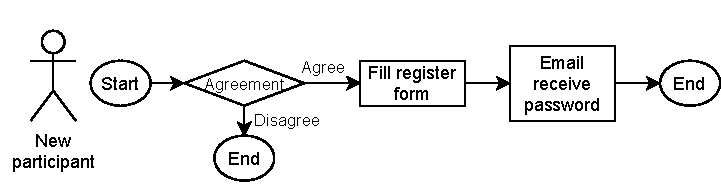
\includegraphics[width=\textwidth]{implementation/imgs/4-webapp-user-register.pdf}
    \caption{New participant registration}
    \label{fig:4-webapp-user-register}
\end{figure}

\begin{figure}[!ht]
    \centering
    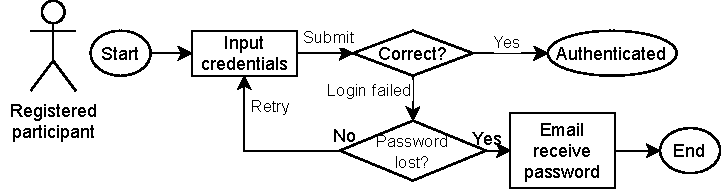
\includegraphics[width=\textwidth]{implementation/imgs/4-webapp-user-login.pdf}
    \caption{Registered participant login}
    \label{fig:4-webapp-user-login}
\end{figure}

\begin{figure}[!ht]
    \centering
    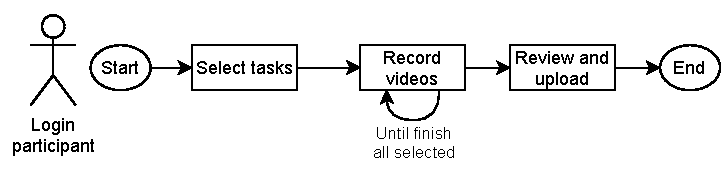
\includegraphics[width=\textwidth]{implementation/imgs/4-webapp-user-record.pdf}
    \caption{Participant recording and uploading}
    \label{fig:4-webapp-user-record}
\end{figure}
